\documentclass[11pt,letterpaper]{article}

\usepackage[margin=0.90in,top=0.92in,bottom=0.92in]{geometry}
\usepackage[utf8]{inputenc}
\usepackage[T1]{fontenc}
\usepackage{newpxtext,newpxmath} % Palatino typography
\usepackage{microtype}
\usepackage{amsmath,amsfonts}
\usepackage{graphicx}
\usepackage{booktabs}
\usepackage{xcolor}
\usepackage{fancyhdr}
\usepackage{enumitem}
\usepackage{titlesec}
\usepackage{tikz}
\usepackage{listings}
\usepackage{hyperref}

% Palette
\definecolor{primaryblue}{RGB}{2, 100, 160}
\definecolor{accentindigo}{RGB}{60, 50, 190}
\definecolor{accentteal}{RGB}{12, 110, 105}
\definecolor{darkslate}{RGB}{28, 38, 52}
\definecolor{warmbg}{RGB}{252, 250, 247}
\definecolor{boxborder}{RGB}{210, 220, 230}
\definecolor{calloutbg}{RGB}{242, 248, 255}
\definecolor{codebg}{RGB}{247, 249, 252}
\definecolor{codeframe}{RGB}{220, 228, 238}

% Hyperref
\hypersetup{
    colorlinks=true,
    linkcolor=accentindigo,
    citecolor=primaryblue,
    urlcolor=accentteal
}

% Section Titles
\titleformat{\section}{\Large\bfseries\color{primaryblue}}{\thesection.}{0.6em}{}[\vspace{-0.3em}{\color{boxborder}\hrule height 0.7pt}]
\titleformat{\subsection}{\large\bfseries\color{accentindigo}}{\thesubsection}{0.6em}{}
\titleformat{\subsubsection}{\normalsize\bfseries\color{darkslate}}{\thesubsubsection}{0.6em}{}
\titlespacing*{\section}{0pt}{5pt plus 1.5pt minus 1pt}{2.5pt plus 1pt minus 1pt}
\titlespacing*{\subsection}{0pt}{3.5pt plus 1pt minus 1pt}{1.5pt plus 1pt minus 1pt}
\setlength{\abovedisplayskip}{3.5pt plus 1pt minus 1pt}
\setlength{\belowdisplayskip}{3.5pt plus 1pt minus 1pt}
\setlength{\abovedisplayshortskip}{2pt plus 1pt minus 1pt}
\setlength{\belowdisplayshortskip}{2pt plus 1pt minus 1pt}

% Headers / Footers
\pagestyle{fancy}
\fancyhf{}
\fancyhead[L]{\small\sffamily\color{darkslate}\textbf{Cultural Mechanics}}
\fancyhead[R]{\small\sffamily\color{primaryblue}\textbf{Lecture 01}}
\fancyfoot[L]{\scriptsize\sffamily\color{darkslate!60}Semantic Mechanics Project $\cdot$ Mathematical Linguistics Group}
\fancyfoot[R]{\small\sffamily\color{darkslate}\thepage}
\renewcommand{\headrulewidth}{0.4pt}
\renewcommand{\footrulewidth}{0.4pt}

% Callout Boxes
\newcommand{\calloutbox}[2]{%
\vspace{0.35em}\noindent
\begin{tikzpicture}
\node[draw=primaryblue, fill=calloutbg, rounded corners=4pt, line width=0.9pt, text width=\dimexpr\linewidth-24pt\relax, inner sep=7.5pt] {
    {\sffamily\bfseries\color{primaryblue}#1}\par\vspace{0.25em}{\color{boxborder}\hrule height 0.5pt}\vspace{0.45em}
    {\small\color{darkslate}#2}
};
\end{tikzpicture}\vspace{0.35em}
}

\newcommand{\socraticbox}[2]{%
\vspace{0.35em}\noindent
\begin{tikzpicture}
\node[draw=accentindigo, fill=warmbg, rounded corners=4pt, line width=0.9pt, text width=\dimexpr\linewidth-24pt\relax, inner sep=7.5pt] {
    {\sffamily\bfseries\color{accentindigo}#1}\par\vspace{0.25em}{\color{boxborder}\hrule height 0.5pt}\vspace{0.45em}
    {\small\color{darkslate}#2}
};
\end{tikzpicture}\vspace{0.35em}
}

% Code Listings Configuration
\lstset{
    backgroundcolor=\color{codebg},
    frame=single,
    rulecolor=\color{codeframe},
    basicstyle=\ttfamily\footnotesize\color{darkslate},
    keywordstyle=\bfseries\color{accentindigo},
    commentstyle=\itshape\color{accentteal},
    stringstyle=\color{primaryblue},
    breaklines=true,
    tabsize=4,
    showstringspaces=false,
    captionpos=b,
    xleftmargin=6pt,
    xrightmargin=6pt
}

% Float Spacing
\setlength{\textfloatsep}{7pt plus 2pt minus 2pt}
\setlength{\intextsep}{5pt plus 2pt minus 2pt}
\setlength{\abovecaptionskip}{3pt}
\setlength{\belowcaptionskip}{3pt}

\begin{document}

% Title Block
\begin{center}
    {\small\sffamily\bfseries\color{darkslate} SEMANTIC MECHANICS PROJECT $\cdot$ MATHEMATICAL LINGUISTICS GROUP}\\[0.7em]
    {\LARGE\bfseries\color{primaryblue} Lecture 01: Representational Genealogy}\\[0.35em]
    {\Large\bfseries\color{primaryblue} Computational Environments and the Politics of Notation}\\[0.4em]
    {\normalsize\sffamily\color{darkslate} \textbf{Course:} Cultural Mechanics $\cdot$ \textbf{Semester:} Autumn 2026}\\[0.25em]
    {\small\sffamily\color{darkslate!80} \textbf{Prerequisites:} Linear Algebra, Theory of Computation, Scientific Python/R}\\[0.25em]
    {\small\sffamily\color{darkslate!80} \textbf{Foundational Readings:} Arthur (1989), Cajori (1928), Babbage et al. (1813), Lambek (1958), Shannon (1948)}
\end{center}
\vspace{0.1em}
\hrule height 1.2pt \vspace{0.7em}

\section{The Foundational Axiom}

Welcome to the Cultural Mechanics, a short book and class on a part of the larger \textbf{Semantic Mechanics Project}. Across computer science, formal linguistics, and pure mathematics, notation is routinely introduced as an incidental, transparent window onto timeless truth. Students are instructed to memorize differential symbols, syntactic parse trees, matrix brackets, and tensor indices as though they were handed down on stone tablets, wholly independent of the physical, economic, and institutional media in which they were inscribed.

This pedagogical myth obscures the central reality of symbolic thought: \textbf{notations are economic technologies}. They are cognitive compression algorithms engineered under severe physical constraints:
\begin{enumerate}[noitemsep,topsep=1pt]
    \item \textbf{Printing and Mechanical Ergonomics:} The physical friction of typefounding, ink smudging, lead casting, keyboard layouts, and screen rendering.
    \item \textbf{Cognitive Coordination and Processing Barriers:} The working memory capacity of the human visual cortex ($\sim 4$ to $7$ chunks) and the algebraic composability of symbolic transformations.
    \item \textbf{Institutional Subsidies and Path-Dependent Monopolies:} The imperial, military, academic, and industrial capital deployed to subsidize specific notations while legislating alternatives out of existence.
\end{enumerate}

\calloutbox{The Axiom of Representational Genealogy}{%
Let $\mathcal{C}$ be a formal conceptual domain (e.g., infinitesimal calculus, grammatical structure, semantic similarity). A symbolic representation $R \in \mathcal{R}_{\mathcal{C}}$ survives not because its abstract fidelity $\Phi(R)$ is maximal, but because it minimizes a composite \textbf{representational cost function}:
\begin{equation}
\mathcal{L}(R) = C_{\text{print}}(R) + C_{\text{cog}}(R) + C_{\text{coord}}(R) - \lambda \cdot \mathcal{S}_{\text{inst}}(R)
\end{equation}
where $C_{\text{print}}$ is reproduction and compiler friction, $C_{\text{cog}}$ is visual-cognitive parsing overhead, $C_{\text{coord}}$ is network switching cost across practitioners, and $\mathcal{S}_{\text{inst}}$ is the capital subsidy supplied by sovereign institutions (academies, defense agencies, standardized educational publishers).
}

When institutional inertia $\mathcal{S}_{\text{inst}}$ dominates, formalisms exhibit \textbf{path-dependent technological lock-in} (Arthur, 1989). A sub-optimal notation can monopolize an entire civilization's intellectual output for centuries, introducing sustained cognitive friction and adoption overhead across generations of practitioners.

\begin{figure}[htbp]
\centering
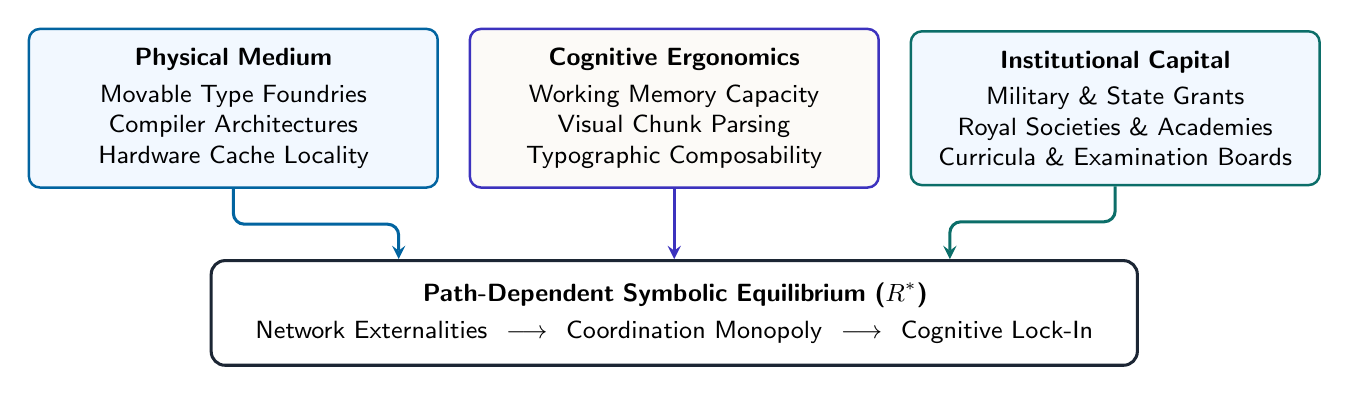
\begin{tikzpicture}[every node/.style={font=\small\sffamily}]
    % Top row boxes with generous, balanced spacing (gap = 7mm)
    \node[draw=primaryblue, fill=calloutbg, rounded corners=4pt, line width=0.9pt, inner sep=7pt, text width=4.7cm, align=center] (tech) at (-5.6, 1.6) {
        \textbf{Physical Medium}\\[0.25em]
        Movable Type Foundries\\
        Compiler Architectures\\
        Hardware Cache Locality
    };
    
    \node[draw=accentindigo, fill=warmbg, rounded corners=4pt, line width=0.9pt, inner sep=7pt, text width=4.7cm, align=center] (cog) at (0.0, 1.6) {
        \textbf{Cognitive Ergonomics}\\[0.25em]
        Working Memory Capacity\\
        Visual Chunk Parsing\\
        Typographic Composability
    };
    
    \node[draw=accentteal, fill=calloutbg, rounded corners=4pt, line width=0.9pt, inner sep=7pt, text width=4.7cm, align=center] (inst) at (5.6, 1.6) {
        \textbf{Institutional Capital}\\[0.25em]
        Military \& State Grants\\
        Royal Societies \& Academies\\
        Curricula \& Examination Boards
    };
    
    % Bottom box with clear vertical clearance and single-line flow
    \node[draw=darkslate, fill=white, rounded corners=5pt, line width=1.1pt, inner sep=8pt, text width=11.2cm, align=center] (lockin) at (0.0, -1.0) {
        \textbf{Path-Dependent Symbolic Equilibrium ($R^*$)}\\[0.25em]
        Network Externalities $\;\longrightarrow\;$ Coordination Monopoly $\;\longrightarrow\;$ Cognitive Lock-In
    };
    
    % Elegant orthogonal connection lines with rounded corners
    \draw[->, >=stealth, line width=1.1pt, color=primaryblue, rounded corners=4pt] (tech.south) -- ++(0,-0.45) -| ([xshift=-3.5cm]lockin.north);
    \draw[->, >=stealth, line width=1.1pt, color=accentindigo] (cog.south) -- (lockin.north);
    \draw[->, >=stealth, line width=1.1pt, color=accentteal, rounded corners=4pt] (inst.south) -- ++(0,-0.45) -| ([xshift=3.5cm]lockin.north);
\end{tikzpicture}
\caption{The Tripartite Economy of Representational Genealogy: physical substrates, cognitive limits, and institutional subsidies jointly dictate symbolic survival.}
\label{fig:genealogy_triad}
\end{figure}

\section{The Computational Laboratory}

Semantic Mechanics is an \textbf{empirical mathematical discipline}. Throughout this course, theoretical claims are matched against executable computational models, corpus simulations, and high-performance vector pipelines. To ensure scientific rigor and platform independence, we maintain a dual-track analytical workbench in both \textbf{Python 3.11+} and \textbf{R}.

\subsection{Virtual Environment Configuration}
All course models must be executed inside isolated virtual environments to prevent dependency contamination. We standardize on Unix-style command environments:

\begin{lstlisting}[language=bash, caption={Laboratory Environment Initialization}]
# 1. Clone the project repository and initialize workspace
git clone https://github.com/Mathematical-Linguistics/semantic-mechanics.git
cd semantic-mechanics

# 2. Python 3.11+ Environment Initialization
python3 -m venv .venv
source .venv/bin/activate
pip install --upgrade pip setuptools wheel
pip install numpy scipy pandas torch matplotlib adjustText ipykernel

# 3. R Track Kernel Verification (Optional for parallel track)
# Rscript -e "install.packages(c('ggplot2', 'dplyr', 'readr', 'IRkernel'), repos='https://cloud.r-project.org')"
# Rscript -e "IRkernel::installspec(name='ir', displayname='R 4.x')"
\end{lstlisting}

\subsection{Hardware-Aware Scientific Computing}
Unlike conventional digital humanities workflows that treat text as small ASCII strings in high-level interpreters, modern cultural dynamics operates over corpora containing hundreds of millions of phonemes and multi-dimensional coordinate projections. We enforce three hardware principles:
\begin{itemize}[noitemsep,topsep=2pt]
    \item \textbf{Memory-Mapped Zero-Copy Streaming:} In Lecture 02 and Notebook 06, we stream 500,000-line vernacular lyric catalogs using POSIX \texttt{mmap}, eliminating garbage collector spikes and memory thrashing.
    \item \textbf{SIMD Vectorization:} Phonetic distance metrics (e.g., Levenshtein phoneme matrices, vowel trajectory angles) are dispatched across CPU vector units (AVX-512 / ARM NEON) via vectorized batch kernels.
    \item \textbf{Deterministic Reproducibility:} Random state initialization must be pinned across all simulation scripts ($s_0 = 42$) to guarantee that numerical phase portraits reproduce identically across operating systems.
\end{itemize}

\section{Corpus Infrastructure and Tabular Schemas}

The empirical foundation of the course rests upon four structured datasets maintained in the repository under \texttt{data/corpus/} and \texttt{models/case\_studies.json}. Every student must understand their schemas and algebraic representations.

\subsection{1. Notational Extinction Dataset (\texttt{data/corpus/notational\_extinction.csv})}
Tracks the historical adoption curve, market share percentage, and institutional survival mechanisms across competing notations from the year 1700 to 2025.
\begin{table}[htbp]
\centering
\small
\begin{tabular}{@{}llllrl@{}}
\toprule
\textbf{Field} & \textbf{Type} & \textbf{Example Value} & \textbf{Theoretical Significance} \\
\midrule
\texttt{system} & String & \texttt{Mathematics} & Symbolic domain subject to competition \\
\texttt{epoch} & Integer & \texttt{1740} & Historical timestamp (calendar year) \\
\texttt{notation} & String & \texttt{Newtonian Fluxions} & Formal notation identifier \\
\texttt{share\_pct} & Float & \texttt{38.0} & Percentage adoption among active practitioners \\
\texttt{domain} & String & \texttt{Calculus (UK)} & Geographic or disciplinary boundary \\
\texttt{retention\_type} & String & \texttt{Doctrinal Monopoly} & Economic / institutional survival mode \\
\bottomrule
\end{tabular}
\caption{Schema for the Notational Extinction Corpus, tracking path-dependent market shares.}
\label{tab:schema_extinction}
\end{table}

\subsection{2. Working Vocabulary Horizon (\texttt{data/corpus/vocabulary\_horizon.csv})}
Calibrates the lexical frontier $V(N)$---the number of unique words deployed across the first $N = 35{,}000$ lyrics or prose words---contrasting vernacular lyrical poets (e.g., Aesop Rock, GZA, Kool Keith) against canonical literary masters (Shakespeare, Melville).
\begin{equation}
V(N) = \sum_{k=1}^N \mathbb{I}[w_k \notin \{w_1, \dots, w_{k-1}\}], \qquad \text{for } N = 35{,}000
\end{equation}
Empirical findings demonstrate that vernacular masters surpass Shakespeare by up to $+42.8\%$ in unique lexical density, falsifying the racist folk-theory that colloquial vernaculars are ``lexically impoverished.''

\subsection{3. Euphemism Treadmill and Durability (\texttt{data/corpus/euphemism\_treadmill.csv})}
Measures the semantic half-life $\tau_{1/2}$ of terms introduced by institutional authorities (clinical, bureaucratic, diagnostic) compared against self-minted vernacular terms. While institutional euphemisms pejorate rapidly under Pinker's Euphemism Treadmill ($\tau_{1/2} \approx 18$--$24$ years), community-rooted terms with structural semantic shields retain persistent positive valuations.

\subsection{4. Practical Laboratory Data Ingestion}
Listing~\ref{lst:data_loader} illustrates standard ingestion and type verification for course datasets in Python:

\begin{lstlisting}[language=python, caption={Empirical Corpus Ingestion and Validation Routine}, label={lst:data_loader}]
import pandas as pd
from pathlib import Path

DATA_DIR = Path("data/corpus")

# Load Notational Extinction Dataset
df_extinction = pd.read_csv(DATA_DIR / "notational_extinction.csv")
assert {"system", "epoch", "notation", "share_pct"}.issubset(df_extinction.columns)

# Load Working Vocabulary Horizon Dataset
df_vocab = pd.read_csv(DATA_DIR / "vocabulary_horizon.csv")
assert (df_vocab["unique_words"] > 0).all()

# Load Euphemism Treadmill Dataset
df_treadmill = pd.read_csv(DATA_DIR / "euphemism_treadmill.csv")
print(f"Loaded {len(df_extinction)} extinction epochs, {len(df_vocab)} authors, {len(df_treadmill)} terms.")
\end{lstlisting}

\section{Unified Mathematical and Formal Notations}

To eliminate ambiguity across lectures, problem sets, and notebooks, Table~\ref{tab:notations} formalizes the mathematical vocabulary of the course.

\begin{table}[htbp]
\centering
\small
\resizebox{\linewidth}{!}{%
\begin{tabular}{@{}lll@{}}
\toprule
\textbf{Symbol} & \textbf{Mathematical Meaning} & \textbf{Operational Context} \\
\midrule
$\Sigma, \Sigma^*$ & Vocabulary alphabet and Kleene closure of token sequences & Corpus tokenization \\
$\mathcal{V}(w) \in [-1, +1]$ & Pragmatic valence / valuation of token $w$ & Sentiment polarity ledger \\
$\mathcal{V}_{\text{inst}}(w)$ & Institutional / clinical valuation assigned by dictionary & Dominant ideological baseline \\
$\mathcal{J}(w) = -\mathcal{V}_{\text{inst}}(w)$ & Algebraic sign inversion operator ($f \mapsto f^{-1}$) & Vernacular semantic reclamation \\
$\mathbf{e}(w) \in \mathbb{R}^d$ & Dense continuous vector embedding of token $w$ & Latent semantic space ($d=300$) \\
$\cos(\mathbf{u}, \mathbf{v})$ & Cosine similarity $\frac{\mathbf{u} \cdot \mathbf{v}}{\|\mathbf{u}\|_2 \|\mathbf{v}\|_2}$ & Directional proximity in embedding space \\
$\mathbf{p}_{\text{virt}}, \mathbf{p}_{\text{path}}$ & Virtuosity and Pathology Attractor Poles in $\mathbb{R}^d$ & Semantic phase portrait poles \\
$T_C(R)$ & Typographical and mechanical transaction cost of notation $R$ & Printing and compilation friction \\
$C_{\text{entry}}(R)$ & Cognitive barrier to entry and working memory overhead & Educational learning curve \\
$F(t) \in [0, 1]$ & Cumulative adoption fraction of notation over time & Bass diffusion dynamics \\
$(P, \le, \cdot, 1, (-)^l, (-)^r)$ & Partially ordered monoid with left/right adjoint inverses & Lambek pregroup grammar \\
$\rho_{\text{pragmatic}}$ & Pragmatic Density Index (Gateian double-voiced ratio) & Information-theoretic cryptographic hardness \\
$\text{MSRD}$ & Multi-Syllabic Rhyme Density ($\frac{\text{Assonant Rhyme Morae}}{\text{Total Syllables}}$) & Phonetic Proof-of-Work \\
$\theta \in [0, 1]$ & Mainstream / commercial institutional saturation & Diffusion saturation parameter \\
$\theta^* \approx 0.35$ & Saturation Inflection Point (critical threshold where $\frac{\partial U}{\partial \theta} < 0$) & Vernacular transition phase \\
\bottomrule
\end{tabular}%
}
\caption{The Master Notational Ledger of Semantic Mechanics.}
\label{tab:notations}
\end{table}

\section{Historical Case Studies in Representational Genealogy}

To operationalize our framework, we investigate two major case studies where the political economy of notation governed centuries of intellectual history.

\subsection{The Calculus Wars}
Between 1684 and 1820, mathematics witnessed the most consequential notational clash in scientific history. Isaac Newton conceptualized the calculus through \textbf{fluxions} ($\dot{x}, \ddot{x}$), treating variables as flowing quantities generated by physical kinematics. Gottfried Wilhelm Leibniz conceptualized the calculus as an \textbf{algebraic ledger of differences} ($\frac{dy}{dx}, \int y\,dx$).

\begin{figure}[htbp]
\centering
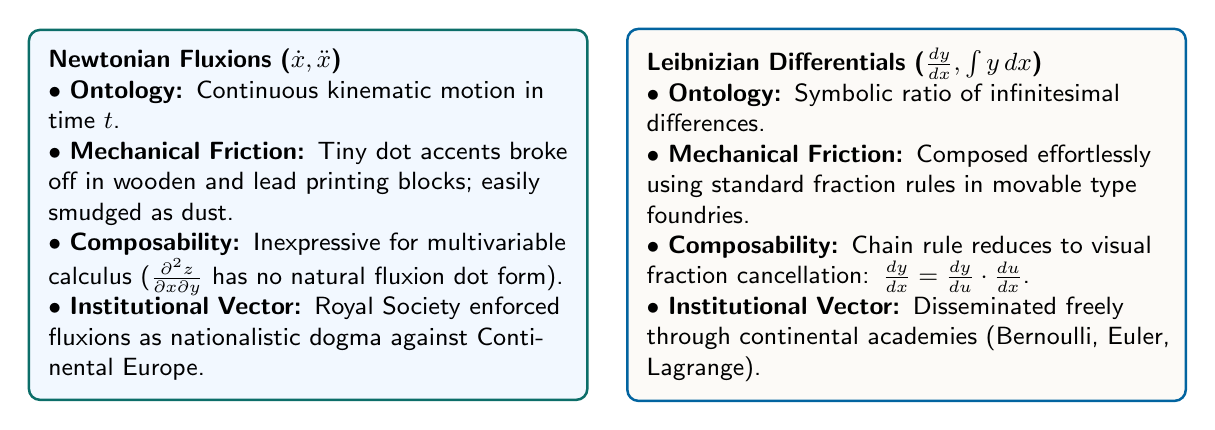
\begin{tikzpicture}[scale=0.95, every node/.style={font=\small\sffamily}]
    % Newton side
    \node[draw=accentteal, fill=calloutbg, rounded corners=4pt, line width=0.9pt, text width=6.6cm, inner sep=7pt] (newton) at (0,0) {
        \textbf{Newtonian Fluxions ($\dot{x}, \ddot{x}$)}\\
        $\bullet$ \textbf{Ontology:} Continuous kinematic motion in time $t$.\\
        $\bullet$ \textbf{Mechanical Friction:} Tiny dot accents broke off in wooden and lead printing blocks; easily smudged as dust.\\
        $\bullet$ \textbf{Composability:} Inexpressive for multivariable calculus ($\frac{\partial^2 z}{\partial x \partial y}$ has no natural fluxion dot form).\\
        $\bullet$ \textbf{Institutional Vector:} Royal Society enforced fluxions as nationalistic dogma against Continental Europe.
    };
    
    % Leibniz side
    \node[draw=primaryblue, fill=warmbg, rounded corners=4pt, line width=0.9pt, text width=6.6cm, inner sep=7pt] (leibniz) at (8.0,0) {
        \textbf{Leibnizian Differentials ($\frac{dy}{dx}, \int y\,dx$)}\\
        $\bullet$ \textbf{Ontology:} Symbolic ratio of infinitesimal differences.\\
        $\bullet$ \textbf{Mechanical Friction:} Composed effortlessly using standard fraction rules in movable type foundries.\\
        $\bullet$ \textbf{Composability:} Chain rule reduces to visual fraction cancellation:
        $\frac{dy}{dx} = \frac{dy}{du} \cdot \frac{du}{dx}$.\\
        $\bullet$ \textbf{Institutional Vector:} Disseminated freely through continental academies (Bernoulli, Euler, Lagrange).
    };
\end{tikzpicture}
\caption{Architectural comparison of calculus notations. Leibniz's notation triumphed because of lower typographical friction and superior cognitive composability.}
\label{fig:calculus_comparison}
\end{figure}

The algebraic superiority of Leibniz's notation becomes transparent in the derivation of the \textbf{chain rule}. Under Leibniz's notation, composition $y = f(u)$ and $u = g(x)$ reduces to the intuitive cancellation of differential ratios:
\begin{equation}
\frac{\Delta y}{\Delta x} = \frac{\Delta y}{\Delta u} \cdot \frac{\Delta u}{\Delta x} \quad \xrightarrow{\Delta x \to 0} \quad \frac{dy}{dx} = \frac{dy}{du} \cdot \frac{du}{dx}
\end{equation}
In Newtonian fluxions, however, the rate of change of $y$ with respect to $x$ required introducing a hypothetical, auxiliary time parameter $t$, writing $\dot{y} / \dot{x}$, and computing kinematic tangents geometrically. This difference imposed severe cognitive friction on students and researchers alike.

The consequence was catastrophic for English mathematics. While Euler, the Bernoullis, d'Alembert, and Lagrange expanded differential calculus into fluid dynamics, analytical mechanics, and variational calculus, British mathematics fell into a 110-year stagnation. The British Royal Society, motivated by personal and geopolitical rivalry, mandated fluxions in university curricula, creating an impenetrable cognitive barrier.

It was not until 1812 that three Cambridge undergraduates---Charles Babbage, John Herschel, and George Peacock---founded the \textbf{Analytical Society}. Their explicit mission, declared with subversive wit, was to advocate for:
\begin{quote}
\itshape
``The principles of pure d-ism in opposition to the dot-age of the university.'' (Babbage, 1864)
\end{quote}
The Cambridge reformers translated Lacroix's differential calculus textbook, systematically replaced fluxion dots with Leibnizian differentials in Tripos examinations, and single-handedly modernized British science. \textbf{The victory of Leibniz was not a victory of truth over falsehood; it was a victory of economic ergonomics over nationalistic institutional lock-in.}

\subsection{Syntactic Architecture}
In 1957, Noam Chomsky introduced generative phrase structure grammars ($S \to NP \ VP$), formalizing sentences as hierarchical syntax trees. Almost concurrently, Joachim Lambek (1958) introduced the \textbf{syntactic calculus}---an algebraic, category-theoretic system where words carry types (e.g., $n$, $s$) equipped with left ($n^l$) and right ($n^r$) directional adjoints, such that grammatical parsing is identical to algebraic multiplication:
\begin{equation}
\text{Transitive Sentence:} \quad n \cdot (n^r \cdot s \cdot n^l) \cdot n \ \longrightarrow \ (n \cdot n^r) \cdot s \cdot (n^l \cdot n) \ \le \ 1 \cdot s \cdot 1 = s
\end{equation}

Why did Chomskyan trees achieve near-universal hegemony across American universities, linguistics departments, and early computer science programs, while Lambek's beautiful algebraic calculus remained an esoteric specialty?

The answer lies in \textbf{Cold War institutional economics and hardware alignment}:
\begin{enumerate}[noitemsep,topsep=1pt]
    \item \textbf{DARPA and Military Funding:} In the late 1950s and 1960s, the MIT Research Laboratory of Electronics (RLE) received massive military machine-translation contracts. Phrase structure trees directly aligned with early von Neumann pushdown automata and compiler parsers (e.g., context-free BNF grammars in Algol 60).
    \item \textbf{Hardware-Era Silicon Alignment:} Computing architectures of the 1960s possessed stack memory perfectly suited for recursive descent tree parsing. Category-theoretic monoidal reductions possessed no silicon counterpart in early vacuum-tube or transistor hardware.
    \item \textbf{Curricular Institutionalization:} Generations of cognitive scientists were trained to equate ``grammatical thought'' with tree branching, creating an institutional barrier that lasted for five decades until quantum computing and tensor network semantics (Coecke et al., 2010) rediscovered Lambek's pregroups.
\end{enumerate}

\section{Pedagogical Roadmap, Laboratory Rubric, and Foundations}

\socraticbox{Discussion Prompt: The QWERTY of the Mind}{%
Consider mathematical notation, programming language syntax (e.g., C/Python vs. APL/Lisp), and algorithmic interfaces. Identify one contemporary formal representation that you suspect survives primarily due to network coordination externalities and institutional subsidies ($\mathcal{S}_{\text{inst}}$) rather than cognitive or computational optimality. How would you quantify the resulting cognitive and computational transaction costs?
}

\subsection{Laboratory Assignment 01}
Students will execute \texttt{notebooks/python/01\_notational\_economics\_diffusion.ipynb} (or the parallel R implementation) to perform the following empirical tasks:
\begin{enumerate}[noitemsep,topsep=1pt]
    \item \textbf{Corpus Ingestion and Trajectory Mapping:} Load \texttt{data/corpus/notational\_extinction.csv} and compute the market share trajectories $F(t)$ of Leibnizian differentials vs. Newtonian fluxions from 1700 to 1840.
    \item \textbf{Bass Diffusion Modeling:} Fit a two-parameter Bass model to the Continental vs. British adoption curves:
    \begin{equation}
    \frac{dF(t)}{dt} = \left(p + q F(t)\right)\left(1 - F(t)\right)
    \end{equation}
    Demonstrate that the imitation parameter $q_{\text{Leibniz}} \gg q_{\text{Newton}}$, quantifying the viral cognitive contagion of fraction cancellation.
    \item \textbf{Transaction Cost Differential:} Compute the typographical transaction cost differential:
    \begin{equation}
    \Delta T_C = T_C(\text{Fluxion}) - T_C(\text{Differential})
    \end{equation}
    demonstrating that dot accents incur higher lead-casting breakage rates ($C_{\text{print}}$) and higher working memory search costs ($C_{\text{cog}}$).
\end{enumerate}

\calloutbox{Core Curriculum Structure: The Two Monograph Arc}{%
\begin{itemize}[noitemsep,topsep=2pt]
    \item \textbf{Lecture 01 (This Monograph):} \textit{Representational Genealogy, Computational Environments, and the Politics of Notation}. Establishes the laboratory toolchain, empirical corpus schemas, foundational mathematical ledger, and institutional path-dependence models.
    \item \textbf{Lecture 02 (Companion Monograph):} \textit{Semantic Inversion: Phonetic Proof-of-Work and High-Performance Cultural Mechanics}. Investigates vernacular autonomy, algebraic sign inversion ($f \mapsto f^{-1}$), multisyllabic rhyme density as proof-of-work, and streaming zero-copy HPC implementations.
\end{itemize}
}

\subsection{The Bridge to Lecture 02}
In this lecture, we have seen how institutional hierarchies enforce representational lock-in through political monopolies and capital subsidies. But what happens when human beings are systematically locked out of institutional capital?

In \textbf{Lecture 02: Semantic Inversion}, we turn from the static archives of European academies to the living, hyper-dynamic frontier of vernacular innovation. We will examine how African American Vernacular English and global hip-hop poetics construct an entirely autonomous economic order---minting semantic inverses ($f \mapsto f^{-1}$), embedding phonetic Proof-of-Work, and defending cultural capital against corporate arbitrage.

\subsection*{References}
\begin{enumerate}[label={[\arabic*]},noitemsep,topsep=1pt]
\small
\item Arthur, W. B. (1989). Competing technologies, increasing returns, and lock-in by historical events. \textit{The Economic Journal}, 99(394), 116--131.
\item Babbage, C. (1864). \textit{Passages from the Life of a Philosopher}. Longman, Roberts, and Green.
\item Cajori, F. (1928). \textit{A History of Mathematical Notations}. Open Court Publishing.
\item Chomsky, N. (1957). \textit{Syntactic Structures}. Mouton \& Co.
\item Lambek, J. (1958). The mathematics of sentence structure. \textit{The American Mathematical Monthly}, 65(3), 154--170.
\item Shannon, C. E. (1948). A mathematical theory of communication. \textit{Bell System Technical Journal}, 27(3), 379--423.
\end{enumerate}

\end{document}
